 %
% problemstellung.tex -- Beispiel-File für die Beschreibung des Problems
%
% (c) 2020 Prof Dr Andreas Müller, Hochschule Rapperswil
%
\section{Die Van der Pol Gleichung
\label{vanderpol:section:vdp_gleichung}}
\rhead{Die Van der Pol Gleichung}
Die Van der Pol Gleichung \eqref{vanderpol:equations:vdp} ist eine {\em nichtlineare} Differentialgleichung zweiter Ordnung. 
\index{nichtlinear}%
Die Nichtlinearität wird durch die Tatsache festgelegt, dass der Koeffizient von $\dot{x}$ nicht linear ist. Tatsächlich sind $x^{2}$ und $x \cdot \dot{x}$ zwei nichtlineare Operationen.

\subsection{Van der Pol Gleichung als Oszillator mit nichtlinearem Widerstand
\label{vanderpol:subsection:RLC}}
\begin{figure}
\centering
\begin{tikzpicture}
\draw
  (0,0) to [short, *-] (0,0)
  to [short, *- ,i=$i(t)$] (1,0)
  to [C, l=$C$] (2,0)
  to [L, l=$L$] (5,0)
  (0,0) to [open, *-, v>=$u_{in}(t)$] (0,-2)
  (0,-2) to [short, *-] (5,-2)
  to [R, l=$R$, v<=$u_R(i(t))$] (5,0);
\end{tikzpicture} 
\caption{RLC-Schaltung mit nichtlinearem Widerstand \label{vanderpol:figures:circuit}}
\end{figure}
In der Abbildung \ref{vanderpol:figures:circuit} steht ein klassischer RLC-Serienschwingkreis. In diesem Fall ist aber der Widerstandswert nicht linear. Dies bedeutet, dass die Beziehung zwischen Spannung und Strom nicht mehr vom Typ $u_R(i) = a \cdot i(t)$ lautet. Es kann jedoch als Polynom dargestellt werden, und zwar in unserem Fall dritter Ordnung anstatt des ersten, wie hier gezeigt: 
\index{Schwingkreis}%
\index{Serienschwingkreis}%
\index{RLC}%
\index{Spannung}%
\index{Strom}%
\index{Widerstand}%
\begin{equation}
u_R(i) = a \cdot i^3 + b \cdot i^2 + c \cdot i + d.
\end{equation}
Eine solche Kennlinie könnte man zum Beispiel mit einer Tunneldiode, einer Anordnung von Feldeffekttransistoren oder Operationsverstärkern erhalten. Die Konstanten könnten auf diese Weise zugeordnet werden:
\index{Kennlinie}%
\index{Tunneldiode}%
\index{Feldeffekttransistor}%
\index{Operationsverstärker}%
\begin{equation*}
a = \frac{R_0}{3 \cdot i_0^2}, \quad c = -R_0, \quad b = d = 0,
\end{equation*}
somit:
\begin{align*}
u_R(i) &= \frac{R_0}{3 \cdot i_0^2} \cdot i^3 - R_0 \cdot i \\ 
&= -R_0 \cdot i_0 \biggl(\frac{i}{i_0} - \frac{1}{3} \biggl(\frac{i}{i_0} \biggr)^3 \biggr).  
\end{align*}
Für die Spannungen $u_{L}(t)$ und $u_{C}(t)$, von Spule bzw. Kondensator, sind aus der Elektrotechnik folgende Zusammenhänge bekannt:
\index{Kondensator}%

\begin{equation*}
u_C(t) = \frac{1}{C} \int_{0}^{t} i(\tau) d\tau, \quad u_L(t) = L \frac{di}{dt}.
\end{equation*}
Die Maschengleichung wird nun nach dem zweiten Kirchhoffschen Gesetz:
\index{Maschengleichung}%
\index{Kirchhoffsches Gesetz}%

\begin{equation}
u_{\text{in}}(t) = u_R(t) + u_C(t) + u_L(t).
\label{vanderpol:equations:kirchoff}
\end{equation}
Unter der Annahme, dass die Spannung $u_{\text{in}}$ eine über die Zeit unveränderliche Grösse ist, d.h. $u_{\text{in}}(t) = U_0$, werden die beiden Seiten der Gleichung \eqref{vanderpol:equations:kirchoff} nach $t$ abgeleitet:

\begin{align}
\frac{dU_0}{dt} &= \frac{d}{dt}(u_R(t) + u_C(t) + u_L(t))\\
0 &= -R_0 \cdot i_0 \biggl(\frac{1}{i_0} \frac{di}{dt} - \frac{1}{3 \cdot i_0^3} \frac{d}{dt} (i(t)^3) \biggr) + \frac{1}{C} i(t) + L \frac{d^2i}{dt^2} \notag \\
0 &= -R_0 \cdot i_0 \biggl(\frac{1}{i_0} \frac{di}{dt} - \frac{1}{3 \cdot i_0^3} \cdot \biggl( 3 \frac{di}{dt} i(t)^2 \biggr) \biggl) + \frac{1}{C} i(t) + L \frac{d^2i}{dt^2} \notag \\
0 &= \frac{d^2i}{dt^2} - \frac{R_0}{L}  \frac{di}{dt} \cdot \biggl(1- \biggl(\frac{i(t)}{i_0}\biggr)^2 \biggr) + \frac{1}{LC} i(t).
\end{align}
Die verschiedenen Konstanten werden wie folgt definiert:
\begin{equation*}
\frac{R_0}{L}=\mu, \quad C=\frac{\mu}{R_0}, \quad i_0 = 1,
\end{equation*}
so folgt die Gleichung:
\begin{equation}
\frac{d^{2}i}{dt^{2}} - \mu (1 - i^{2}) \frac{di}{dt} + i = 0.
\label{vanderpol:equations:vdp_i}
\end{equation}
Es ist daher gezeigt, welche Art von System durch diese Differentialgleichung beschrieben werden könnte.

\noindent Offensichtlich gibt es viele Möglichkeiten, diese Art von Nichtlinearität für den Spannungswert $u_R(t)$ zu erreichen, einige sind oben aufgelistet.
Wenn versucht wird, die gleiche Gleichung zu lösen, aber mit einem konstanten $R$ Wert, erhalten wir eine Differentialgleichung des Typs
\begin{equation}
\frac{d^{2}i}{d t^{2}}+\frac{R}{L} \frac{d i}{d t}+\frac{1}{LC}i = 0.
\end{equation}
Sie kann umgeschrieben werden als
\begin{equation}
\frac{d^{2}i}{d t^{2}}+ 2\zeta \frac{d i}{d t}+\omega_0^{2}i = 0,
\end{equation}
wobei $\omega_0$ die Resonanzfrequenz und $\zeta$ die Dämpfungskonstante sind. Die analytische Lösung ist
\index{Resonanzfrequenz}%
\index{Dämpfungskonstante}%
\begin{equation}
i(t) = e^{-\zeta t} \cos(\omega_dt+\varphi_0).
\end{equation}
Das bedeutet, dass im Falle der Gleichung \eqref{vanderpol:equations:vdp_i}, d.h. die Van der Pol Gleichung eine Schwingung vorliegt, die bei grossen Werten von $i^2$ einen positiven Dämpfungswert hat, der ihre Amplitude verringert. Bei kleinen Werten von $i^2$ ist der Dämpfungswert negativ, was dazu führt, dass die Amplitude grösser wird und somit in diesen beiden Zuständen schwingt.

\subsection{Homogene Gleichung
\label{vanderpol:subsection:homogene}}
\index{homogen}%
Die Differentialgleichung wird als homogen bezeichnet, wenn die rechte Seite auf Null gesetzt ist, d.~h. ohne Störfunktion. Sie wird daher wie folgt beschrieben:
\index{Störfunktion}%
\begin{equation}
	\ddot{x} - \mu \left(1-x^{2}\right)\dot{x}+x = 0.
\label{vanderpol:equations:homogene}
\end{equation}
Es ist möglich, die Gleichung mit der folgenden Substitution auf den ersten Grad zu reduzieren wie im Kapitel \ref{buch:section:dglproblemstellung} schon beschrieben. Die Reduktion ist
\index{Reduktion der Ordnung}%
\begin{equation}
\frac{d}{dt}\begin{pmatrix}x \\ y\end{pmatrix} = \begin{pmatrix}y \\ \mu \left(1-x^{2}\right)\dot{x}-x\end{pmatrix}.
\label{vanderpol:equations:homogene_1}
\end{equation}
Die Lösung der Differentialgleichung neigt unabhängig vom Anfangswert dazu, nach einer bestimmten Zeit in einer bestimmten Trajektorien zu oszillieren. Diese Orbit wird Grenzzyklus oder {\em limit cycle} genannt. Mit dem Parameter $\mu$ wird die Form der Umlaufbahn verändert, wie in Abbildung \ref{vanderpol:figures:homogene} dargestellt. Es ist interessant zu bemerken, dass bei $\mu = 0$ die Gleichung zu $\ddot{x} + x = 0$ wird, also eine linear harmonische Schwingung.
\index{Grenzzyklus}%
\index{limit cycle}%
\begin{figure}
	\centering
	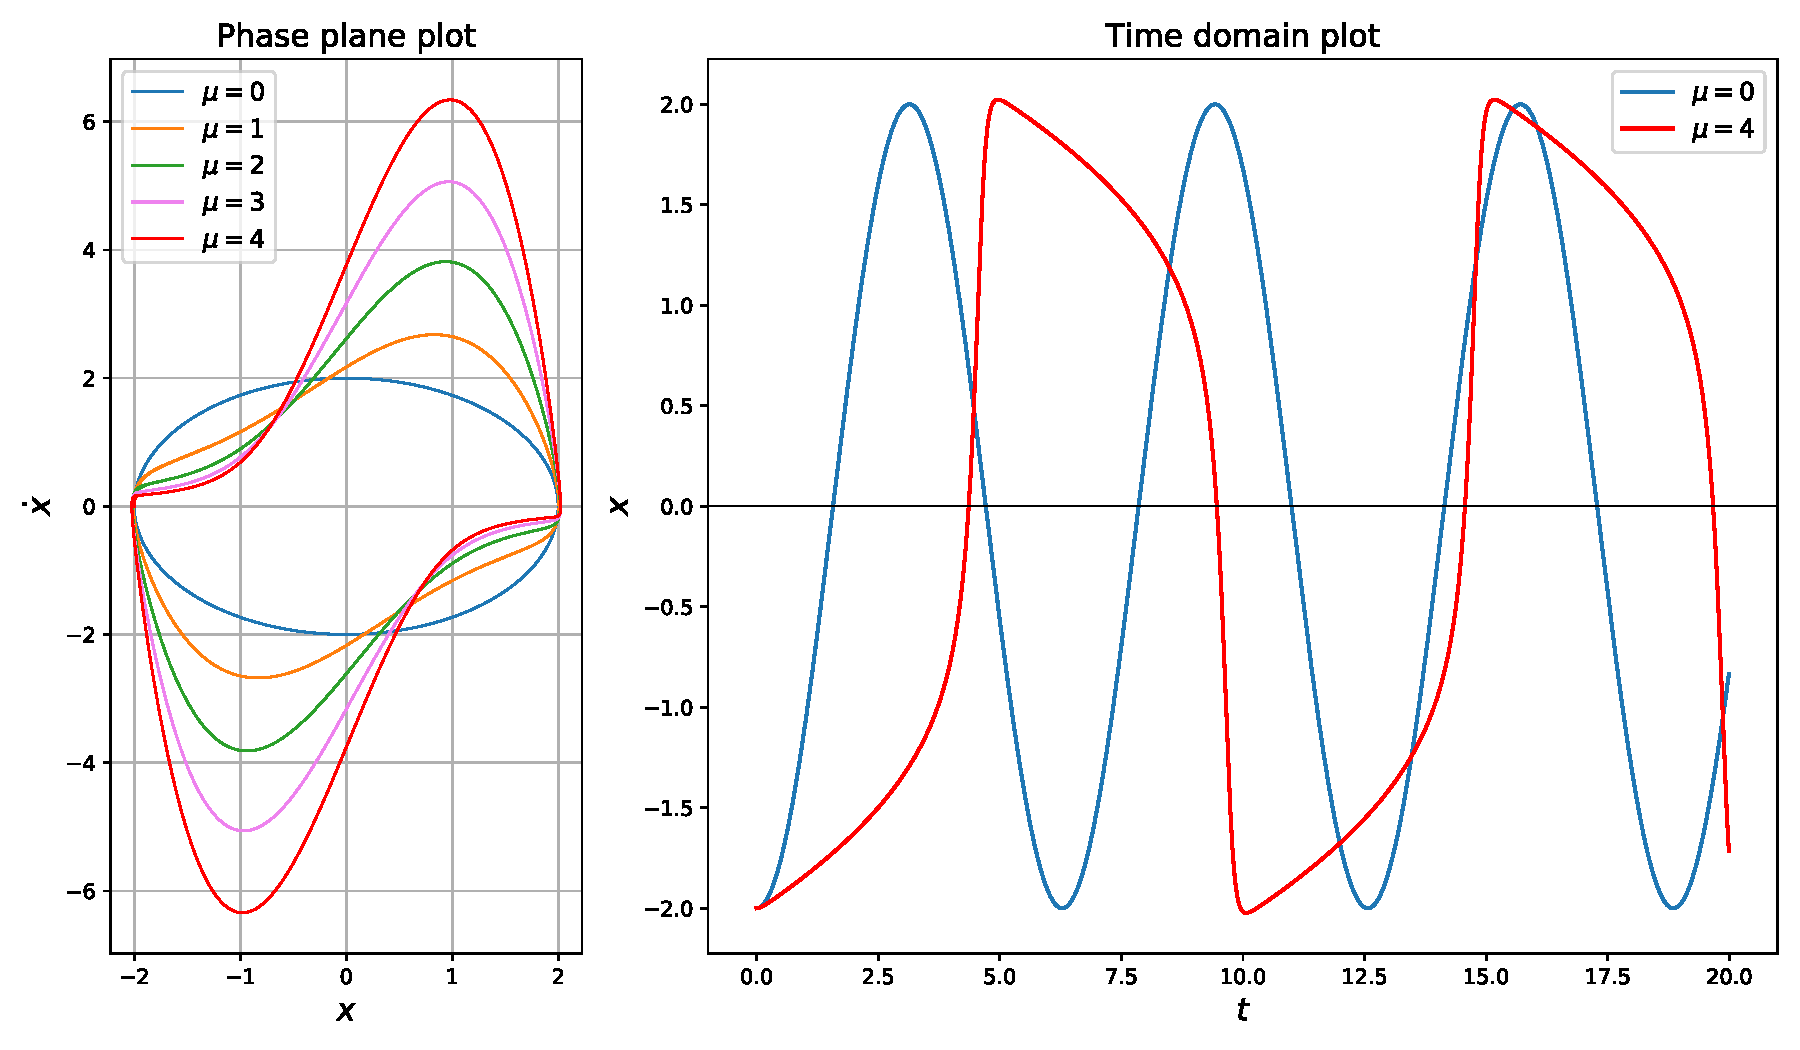
\includegraphics[width=\textwidth]{papers/vanderpol/figures/homogene_plot.pdf}
	\caption{Phase und Zeit Raum Diagramm der Gleichung \eqref{vanderpol:equations:homogene_1} mit verschiedenen Werten von $\mu$\label{vanderpol:figures:homogene}}
\end{figure}
Die homogene Van der Pol Gleichung ist stabil und zeigt {\em kein} chaotisches Verhalten.
\subsection{Inhomogene Gleichung}
\label{vanderpol:subsection:inhomogene}
Die inhomogene Form der Van der Pol Gleichung
\begin{equation*}
	\ddot{x}-\mu(1-x^{2}) \dot{x}+x = f(t),
\label{vanderpol:equations:inhomogene_gen}
\end{equation*}
wird die sogenannte {\em angeregte Van der Pol Gleichung}. In unserem Fall wird die Störfunktion auf $f(t) = A \cdot \sin(\omega t)$ gesetzt:
\index{angeregte Van der Pol-Gleichung}%
\index{Van der Pol-Gleichung!angeregte}%
\begin{equation}
	\ddot{x}-\mu(1-x^{2}) \dot{x}+x = A \cdot \sin(\omega t).
\label{vanderpol:equations:inhomogene_sin}
\end{equation}
Aus praktischer Sicht ist es so, als würde man einen Wechselstromgenerator an den Oszillatoreingang anschliessen. Wie in der Gleichung \eqref{vanderpol:equations:homogene_1}, wird die Differentialgleichung auf die erste Ordnung reduziert:
\begin{align}
\frac{d}{dt}\begin{pmatrix}x \\ y\end{pmatrix} = \begin{pmatrix}y \\ \mu (1-x^{2})frac{dx}{dt}-x+A \cdot \sin(\omega t)\end{pmatrix}.
\label{vanderpol:equations:inhomogene_2}
\end{align}
